\subsubsection{Levelmengen}
\textbf{Definition}\\
\begin{flalign}
    &f^{-1}(\{L\}) = \{p \in A | f(p) = L\}&
\end{flalign}\\
\textbf{Anleitung}\\
\begin{multicols}{2}
    \begin{enumerate}
        \item Level von L bestimmen $f(x,y) \stackrel{!}{=} L$
        \item Nach einer Variablen auflösen (x/y)
        \item Definitionsbereich $\mathbb{D}$ bestimmen
        \item L definieren
        \item Höhenlinien einzeichnen
    \end{enumerate}
\end{multicols}
\textbf{Beispiel}\\
\begin{multicols}{2}
    \begin{flalign*}
        &f(x,y) = x^2 + y^2&\\
        &\boxed{1}: x^2 + y^2 \stackrel{!}{=} L&\\
        &\boxed{2}: y^2 = L - x^2&\\
        &y = \pm \sqrt{c - x^2}&\\
        &\boxed{3}: \mathbb{D} \Rightarrow c - x^2 \ge 0 \Leftrightarrow c \ge x^2&\\
        &\boxed{4}: L = \{0.5; 0.75; 1\}&\\
    \end{flalign*}
    $\boxed{5}$
    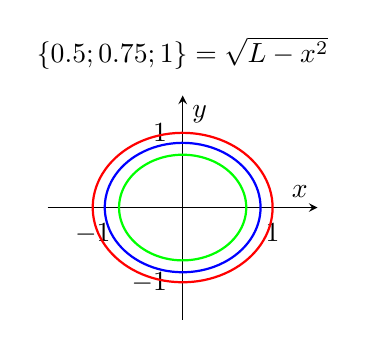
\begin{tikzpicture}
    \begin{axis}[
        scale=0.5,
        axis lines=middle,
        xlabel=\(x\),
        ylabel=\(y\),
        xmin=-1.5, xmax=1.5,
        ymin=-1.5, ymax=1.5,
        samples=100,
        title={$\{0.5;0.75;1\} = \sqrt{L - x^2}$}
    ]
    \addplot[red, thick, domain=0:360] ({cos(x)}, {sin(x)});
    \addplot[green, thick, domain=0:360] ({sqrt(0.5) * cos(x)}, {sqrt(0.5) * sin(x)});
    \addplot[blue, thick, domain=0:360] ({sqrt(0.75) * cos(x)}, {sqrt(0.75) * sin(x)});
    \end{axis}
    \end{tikzpicture}
\end{multicols}